% Kapitel 1 - Einleitung
\section{Introduction}

%In diesem Kapitel wird zunächst die Motivation für dieser Arbeit dargelegt. Danach wird auch auf die Zielsetzung eingegangen, die das Thema der Arbeit fokussiert und den Grundstein für das weitere Vorgehen definiert.

\begin{quote}
    \large "The best or nothing at all." - Gottlieb Daimler
\end{quote}

This famous quote from the automotive industry resonates with every automotive enthusiast, engineer and prospective customer. From the moment we drive our cars off the dealership shop, we rely on various services in-built into the car as well as external services such maintenance checks to keep them running smoothly. Automotive industry, the world over, has come a long way since it's conception in the 19th Century and has taken giant strides in improving passenger safety, comfort and reliability. 

The automotive industry is constantly evolving and improving, which is a result of consistent improvements and developments in the automotive testing. Automotive testing is an essential aspect of the automotive industry, ensuring the safety and reliability of vehicles on the roads. With the increasing complexity of modern vehicles, it is crucial to subject them to thorough testing procedures before they are made available to consumers. This includes testing for a wide range of parameters such as performance, fuel efficiency, emissions, and crash-worthiness. Cars are becoming more and more complex products requiring a lot of effort and investments. \cite{jpower} said that: ”Automakers are investing billions of dollars into designing and building vehicles and adding technologies that consumers desire and demand”.
In order to fulfill the customer needs, modern cars, e.g., the 2014 Audi A8, have up to 80 or 90 Electronic Control Unit (ECU) for realizing the high amount of requested functions, ranging from simple interior lightning up to Advanced Driver Assistance Systems (ADAS) like Adaptive Cruise Control (ACC) \cite{Audi}.

\begin{figure}[H]
    	\centering
    	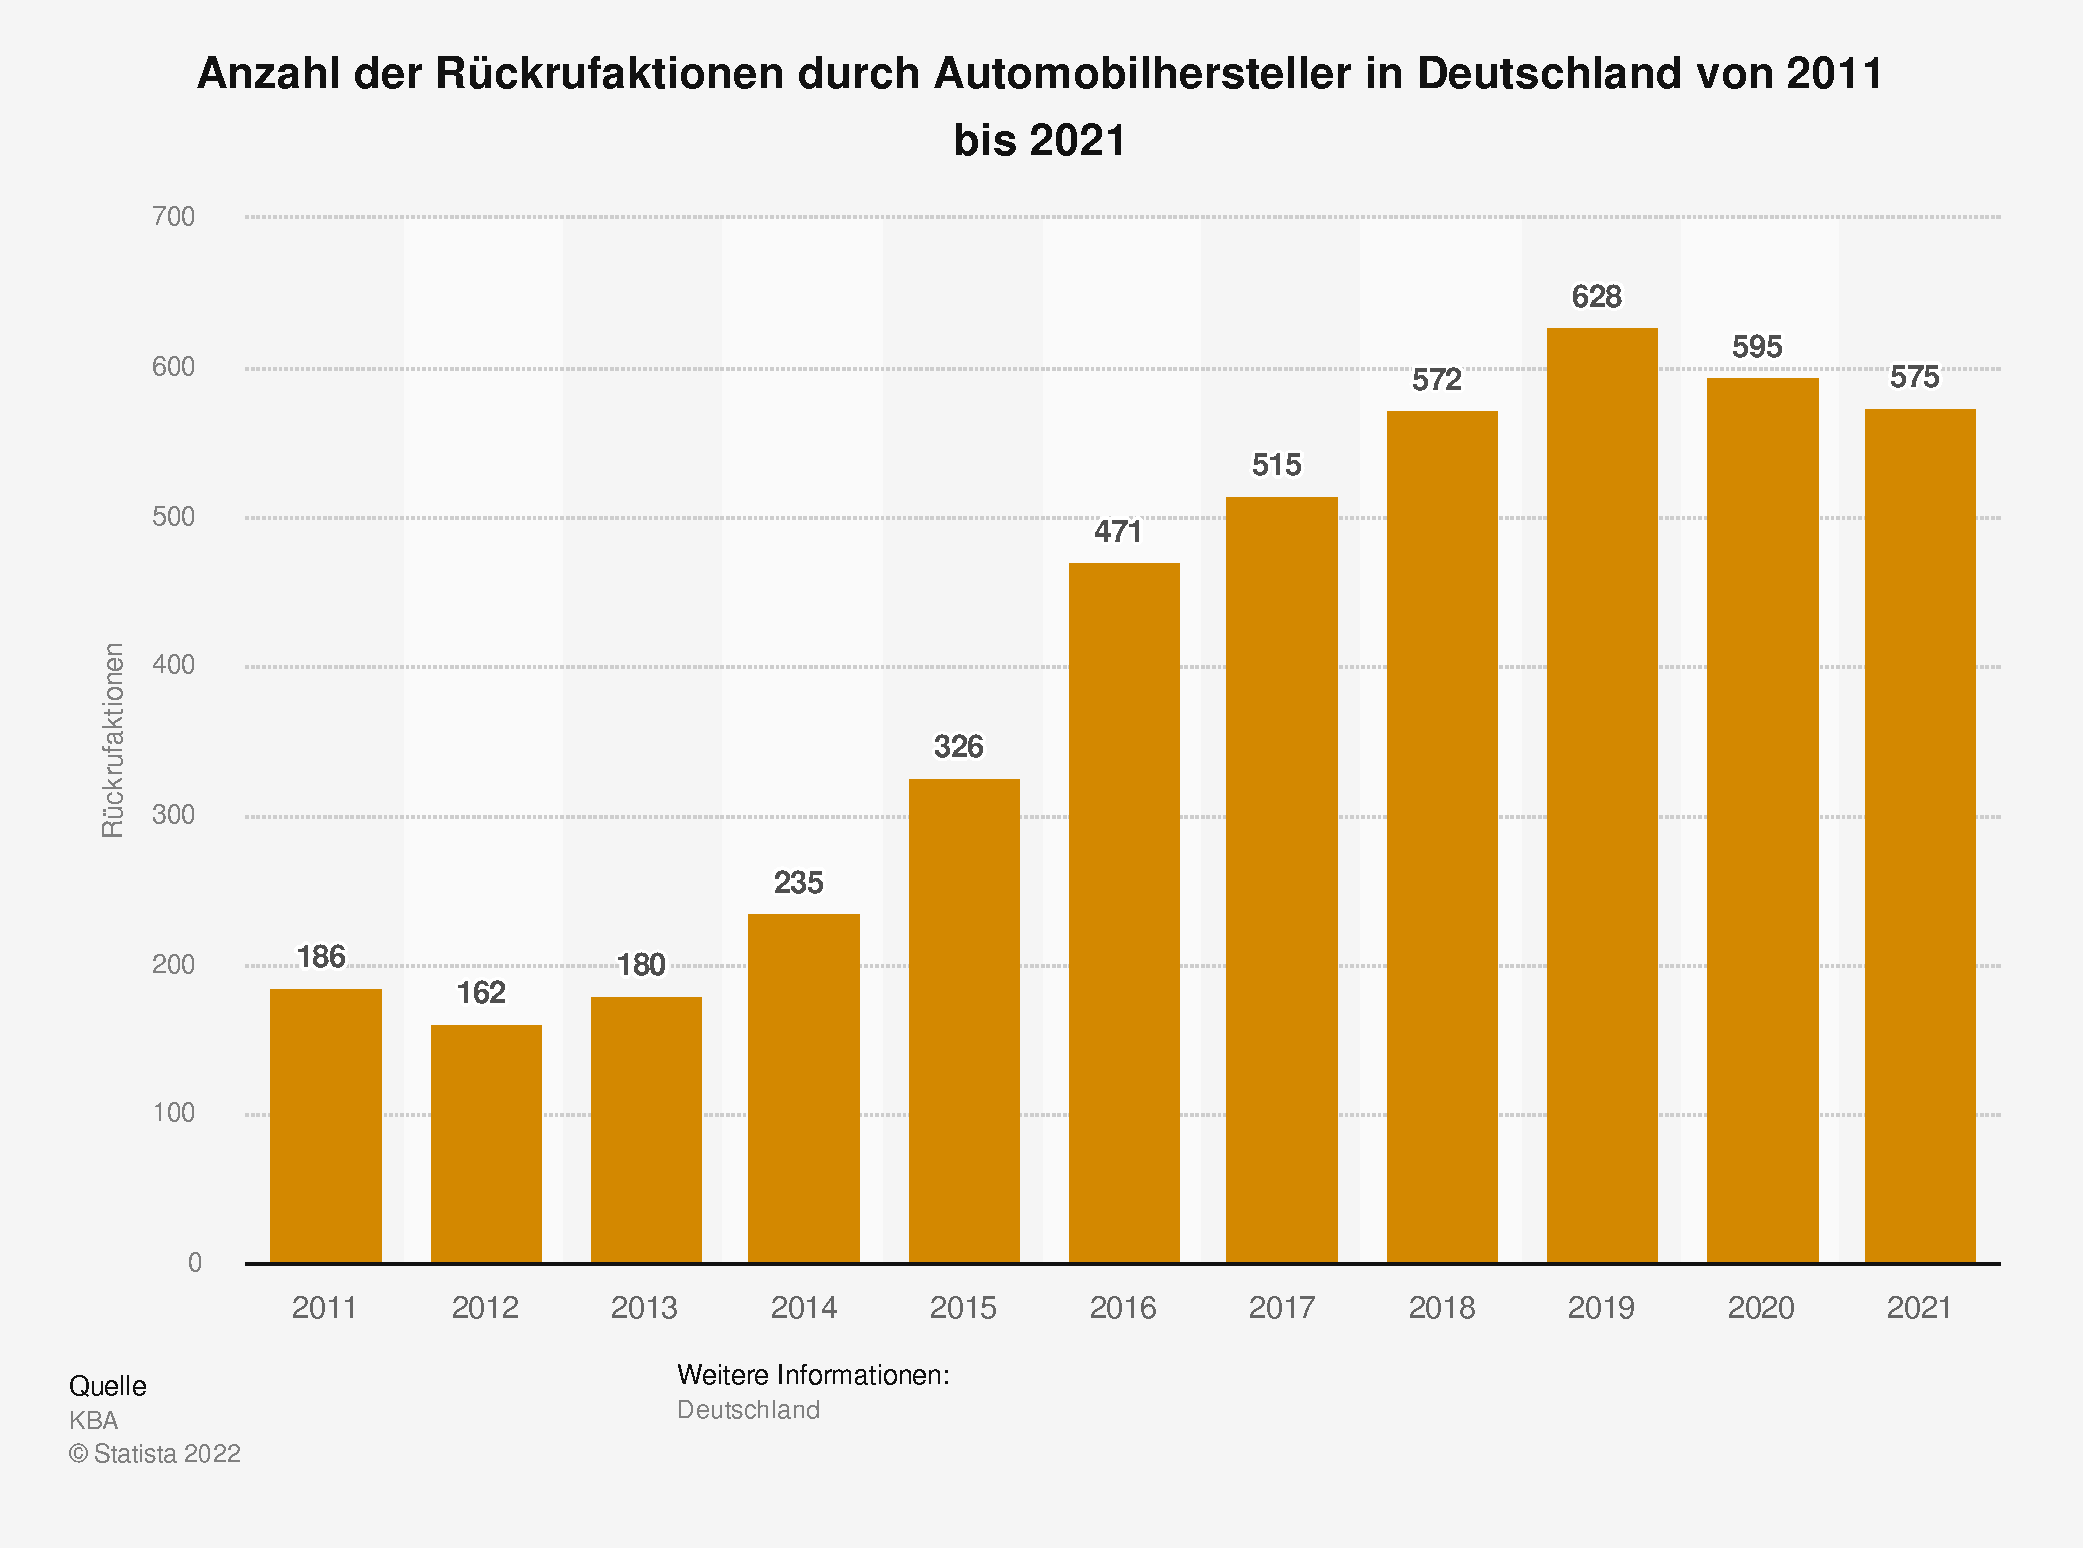
\includegraphics[width= 0.85\textwidth]{images/statistic_id1254342_rueckrufaktionen-in-der-automobilindustrie-in-deutschland-bis-2021.pdf}
    	\caption [Vehicle Recall Data]{ No. of Vehicle Recall Campaigns in Germany 2011-2021; Source: \protect\cite{KBA}}  
    	\label{fig:Statista Data}
\end{figure}
\newpage
The above diagram shows the amount of vehicle recall campaigns in Germany by Automobile Manufacturers between 2011-21. As visible, with increasing complexity and advancements in technology the amount of recalls have also increased. Testing helps manufacturers determine the necessary changes pre-production in order to incur the least damages in form of product recalls. But how do these professionals ensure that changes are necessary or unnecessary?
\textbf{By gathering data, of course!} on which this study is primarily focused on. But before diving deep into data, let's understand a bit about testing. 

Automotive testing plays a key role in the development and improvement of new technologies, such as autonomous driving and electrification. The higher the amount of comfort functions and reliability, the more complex the vehicle is. These vehicles have to undergo various tests to ensure flawless production. The value of testing is often underestimated, not understood, or mostly an afterthought, but it can be the difference between success and failure. The focus is almost always on innovations and developing the best and most sophisticated features for end users. But the questions that should be asked are  — what would these innovations and great features be like if they didn't work as expected? Not usable, not fast enough, not available, not safe — what impact would neglecting quality present? One well-known consequence is OEM mass recall — this can significantly impact people’s lives and the company reputation, plus there’s the financial damage, and the internal impact of diminished team spirit, project escalation, team dissatisfaction, productivity reduction and talent loss. In short, testing is necessary to get the desired results of innovation \cite{luxoft}.

One of the key challenges in automotive testing is simulating real-world conditions as closely as possible. This includes testing vehicles in various weather conditions, at different altitudes, and on different road surfaces. Automotive testing laboratories are equipped with advanced testing equipment and facilities to replicate these conditions and assess the performance of vehicles under a variety of scenarios. These tests fall in the scope of Environmental testing or Environmental Qualifications. Environmental testing also helps demonstrate compliance of your products with international regulations, making it easier to access global markets. Environmental testing also boosts trust in your products \cite{tüv}. In general, environmental tests demonstrate that your products have the build quality to work perfectly, no matter what the conditions. During testing, possible weaknesses can be identified and product improvements can be initiated at an early stage. 

For the purpose of environmental tests, environmental test chambers are used. They simulate various conditions that automotive components might endure in their lifetime. The systems that run such tests are called lifetime tester systems or End-of-life Test systems. Endurance tests, also known as accelerated life tests (ALTs), are a type of reliability testing used to evaluate the lifespan of a product under accelerated conditions. These tests are designed to simulate real-world usage and to identify potential failure points in a product. Endurance tests are often used in the automotive, aerospace, medical, and electronics industries to ensure the reliability of products and to identify potential failure points before they occur in the field. This can result in significant cost savings by identifying issues early in the development process, before mass production begins. In addition to identifying potential failure points, endurance testing can also be used to improve the design of a product. The results of endurance tests can be used to optimize a product's design and materials to increase its lifespan.

Overall, endurance tests or ALTs are an important aspect of product development and reliability testing, ensuring that products are safe, reliable, and able to withstand the rigors of real-world usage. They provide valuable information about a product's expected lifespan and potential failure points, helping companies to improve the design of their products and to increase customer satisfaction. This results in complex and intrinsic testing strategies which in turns results in enormous amounts of test data. Most of the data are desirable while some are undesired. One important aspect of this evolution is the development of effective methods for acquiring data about the environmental performance of vehicles. Environmental endurance tests for automotive components are critical for ensuring the safety and reliability of vehicles on the road. These tests simulate real-world conditions such as extreme temperatures, humidity, and vibration to evaluate the lifespan of components and identify potential failure points. However, the data generated from these tests can be large and complex, making it challenging to manage and analyze. One common problem faced when working with large data sets from environmental endurance tests is the difficulty in identifying patterns or trends in the data. Another problem is that the data can be highly variable, making it difficult to establish clear cause-and-effect relationships. Additionally, the data obtained from these tests is often not in a format that is easy to work with, requiring data processing and cleaning to be able to analyze them. This can be a time-consuming and tedious process.

The size of data log files generated from environmental endurance tests can be quite large, and managing and analyzing them can be a challenge. Here are a few ways to tackle the problem of large data log files:

\begin{itemize}
    \item Data Compression
    \item Data Sub-sampling
    \item Data Filtering
    \item Data management tools
    \item Data archiving
\end{itemize}

This thesis would study some of the above mentioned methods apart from combining approaches of data analytics and data reduction to enhance the efficiency and accuracy of data acquisition for automotive environmental qualifications.

\subsection{Motivation}
%https://www.cbtnews.com/consumer-reports-releases-annual-reliability-rankings-for-auto-brands/
According to \cite{viewpoint} "Reliability testing, aka endurance or durability testing, runs the part through many hours of use while monitoring (sometimes continuously, sometimes periodically), the performance of the part. Different than design validation, the part is usually not subject to a wide range of extreme conditions to look for corner cases, but rather subjected to “normal” operation in an accelerated fashion. Note that “normal” might not imply static operating conditions. Rather the part might be cycled through a range of conditions seen in normal usage, such as back and forth motion for a car seat cushion, or -120 C to +120 C temperature cycling for a satellite part orbiting the earth. Parts are often run to failure or to degraded performance to verify that one design is better or worse than another. Sometimes, the performance measurements are coupled with an analysis of the failure mode(s). Other times, this failure mode and effects analysis (FMEA) is done without reviewing any measurements taken during the cycling, implying that the reliability test system controls the automated cycling without assessing operation. However, starting in the early ~2000s, data collection during cycling has become nearly universal."

When the part is expensive or the cost of failure of the part is expensive the hardware or DUT is more likely to go through non-negligible reliability testing. Often such tests require to mimic the lifetime behaviour of the equipment in discussion. The result is potentially massive amount of data. One could imagine such tests to often run for 100s of hours on average. Depending on the data being collected, and it's type the accumulated data could often end up being 100s of GBs of data. Scaling up the tests and the no. of DUTs tested, a couple of these tests are sufficient to overload the storage infrastructures of companies performing such tests. As explained in previous section, there is great need for efficiently managing the data in order to efficiently reduce the costs but more importantly deliver precise and tangible data to the client.

The Business Center Verification and Validation at CES is responsible for such endurance / life cycle tests. The HiL test-benches are capable of testing up to 8 DUTs at a time. The average duration for such tests are ~250 hours and above. This leads to an accumulation of data to the tune of approx. 500 gb per project. Considering the increasing demands of testing in modern automotive, the massive size of data is a pain point for the IT infrastructure. Apart from the sheer size of data costing the company in terms of storage space and it's scaling, managing such a huge set of data would be a nightmare if the client requests only specific section of data as final result from the tests. This scenario immediately brings two requirements to one's attention :

\begin{itemize}
    \item Reduction of data size
    \item Making sense of the acquired data
\end{itemize} 

The above requirements are the motivation behind the scientific study undertaken with this thesis where the focus lies on designing an algorithm that reduces the size of the acquired data while also attempting to improve the efficiency of data acquisition. 


\begin{comment}
    \begin{figure}[H]
    	\centering
    	\includegraphics[width= 0.95\textwidth]{}
    	\caption[Verlauf der Anzahl an Todesopfer im deutschen Straßenverkehr von 1953 bis 2016 in Kombination mit Einführung von Fahrerassistenzsystemen]{Statistik der Todesfälle im deutschen Straßenverkehr mit Einführungsdaten von FAS; Quelle: Statistisches Bundesamt \protect\cite{sba}}  
    	\label{fig:Statista Data}
    \end{figure}
\end{comment}
\begin{comment}



















\subsection{Zielsetzung}
\glqq Die Automatisierung der Fahrzeugführung verändert die Anforderungen an das kognitive System des Autofahrers grundlegend. Um daraus keine Gefahren entstehen zu lassen, sind noch zahlreiche Fragen offen.\grqq{} \cite{schlott}. Schlott trifft diese Aussage um die kritischen Aspekte der hochautomatisierten Fahrt zu beleuchten und um auf mögliche Risiken hinzuweisen. 

Diese Arbeit befasst sich sowohl mit der Erhebung der technischen Grundlagen, als auch mit dem menschlichen Informationsverarbeitungsprozess. Die Erkenntnisse aus den einzelnen Bereichen werden aggregiert und miteinander verknüpft, um somit die Basis für ein umfassendes HMI-Konzept zu generieren. Dieses soll die benötigten Informationen aller Automatisierungsstufen zur Förderung des Vertrauens in das Gesamtsystem und Aufrechterhaltung des Situationsbewussteins darstellt, um den Fahrer zu unterstützen. 

Das auszuarbeitende Konzept soll in einem Entwicklungsfahrzeug, weitere Details siehe \autoref{sec:entfahr}, eingesetzt werden und umfasst somit nur die Automatisierungsstufen 0 bis 3, da zum aktuellen Zeitpunkt noch keine aktiven Fahrerassistenzsysteme für höhere Automatisierungsstufen zur Verfügung stehen. Dazu wird folgende Forschungsfrage gestellt: \\

\begin{tabular}{p{0.3cm} p{0.5cm} p{13cm} p{0.5cm}}
	& \textbf{RQ}	& Können die bla bla? & \\
\end{tabular}
\vspace{1em} 

Es wird angenommen, dass sich das Informationsbedürfnis des Fahrers über die Automatisierungsstufen unterschiedlich verhält und eine sich dynamisch veränderbare Anzeige gefordert wird. Daraus lassen sich folgende Hypothesen ableiten: \\

\begin{longtable}{p{0.3cm} p{0.5cm} p{13cm} p{0.5cm}}
	& \textbf{H1}	& Je höher, desto geringer. & \\
	& & & \\
	& \textbf{H2}	& Bla bla, bla bla. & \\
	& & & \\
	& \textbf{H3}	& Bla bla, bla bla. & \\
\end{longtable}
\end{comment}